\section{Sub\-Bar\-Album\-Clock Class Reference}
\label{classSubBarAlbumClock}\index{SubBarAlbumClock@{SubBarAlbumClock}}
{\tt \#include $<$subbaralbumclock.h$>$}

Inheritance diagram for Sub\-Bar\-Album\-Clock:\begin{figure}[H]
\begin{center}
\leavevmode
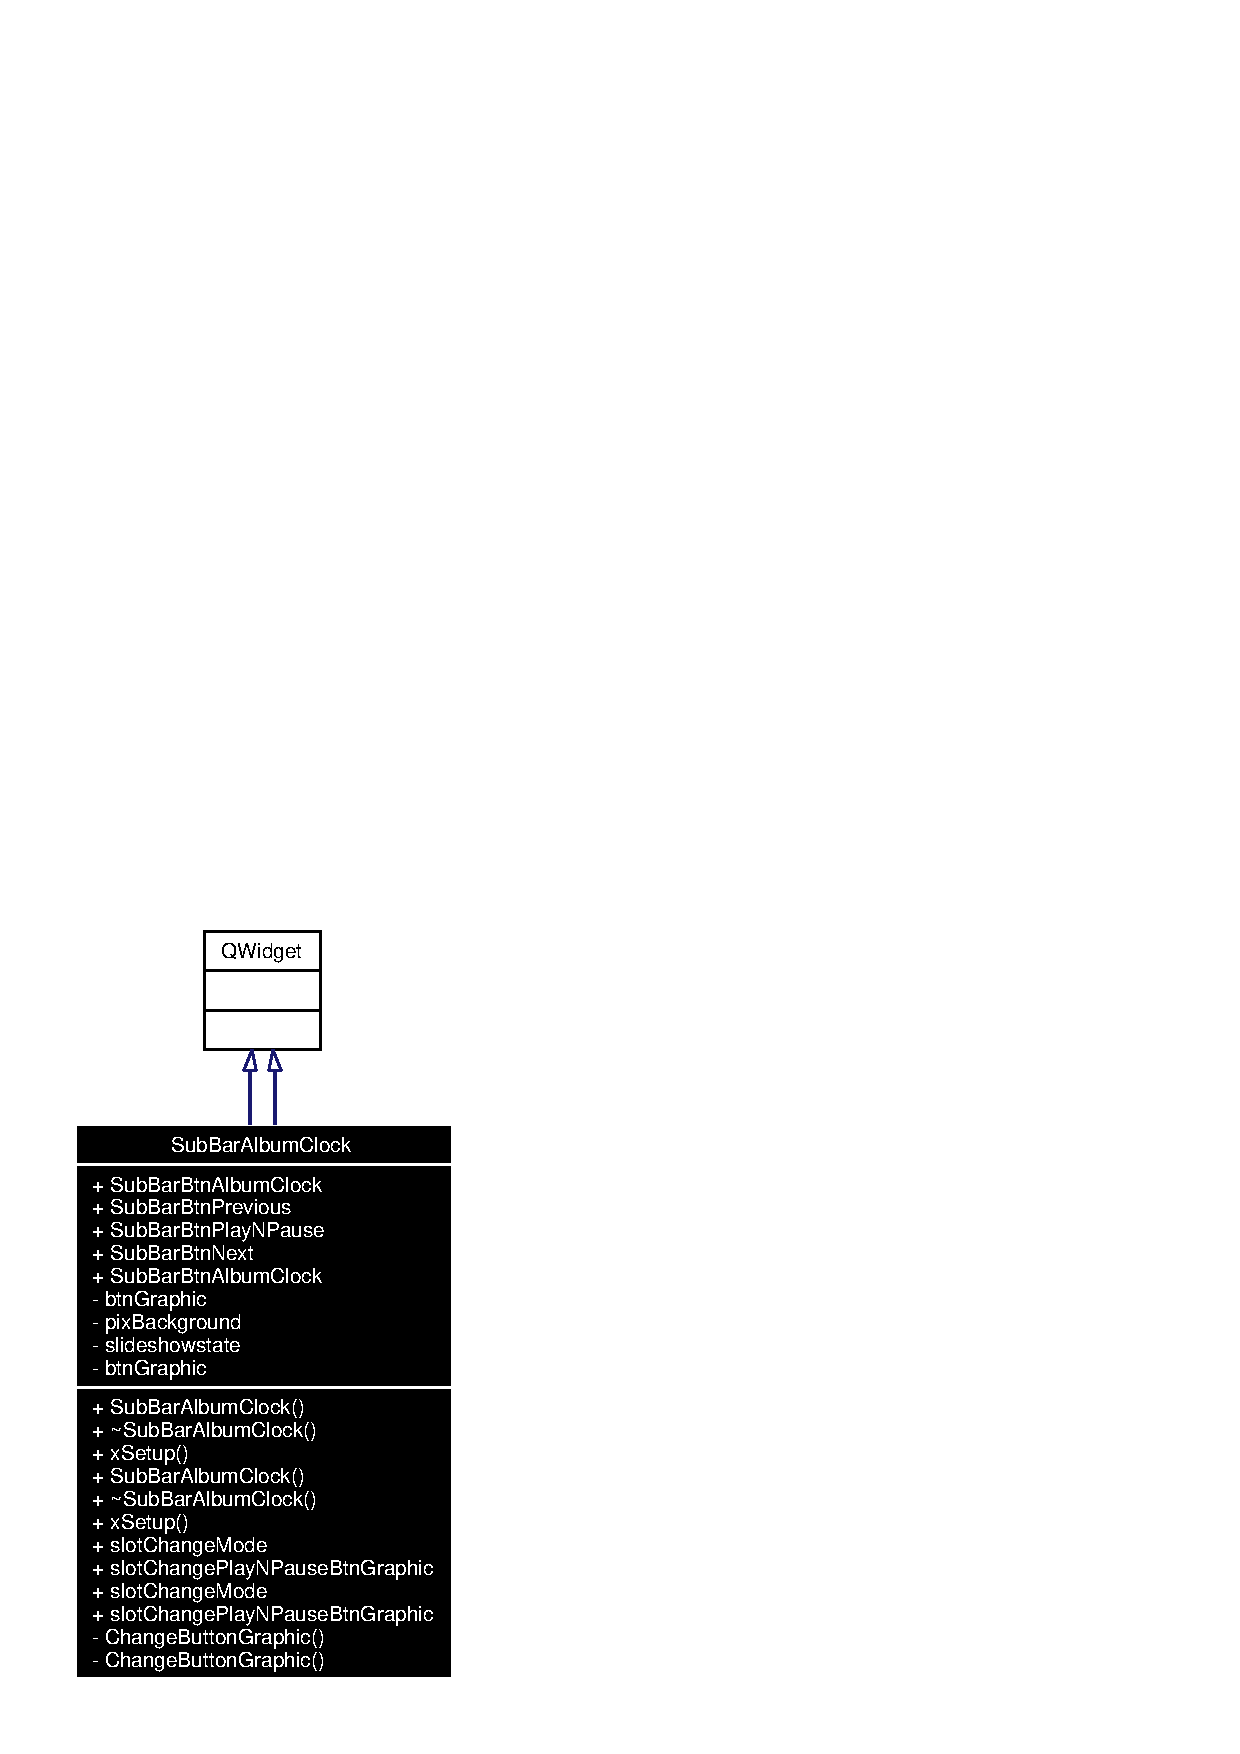
\includegraphics[width=108pt]{classSubBarAlbumClock__inherit__graph}
\end{center}
\end{figure}
Collaboration diagram for Sub\-Bar\-Album\-Clock:\begin{figure}[H]
\begin{center}
\leavevmode
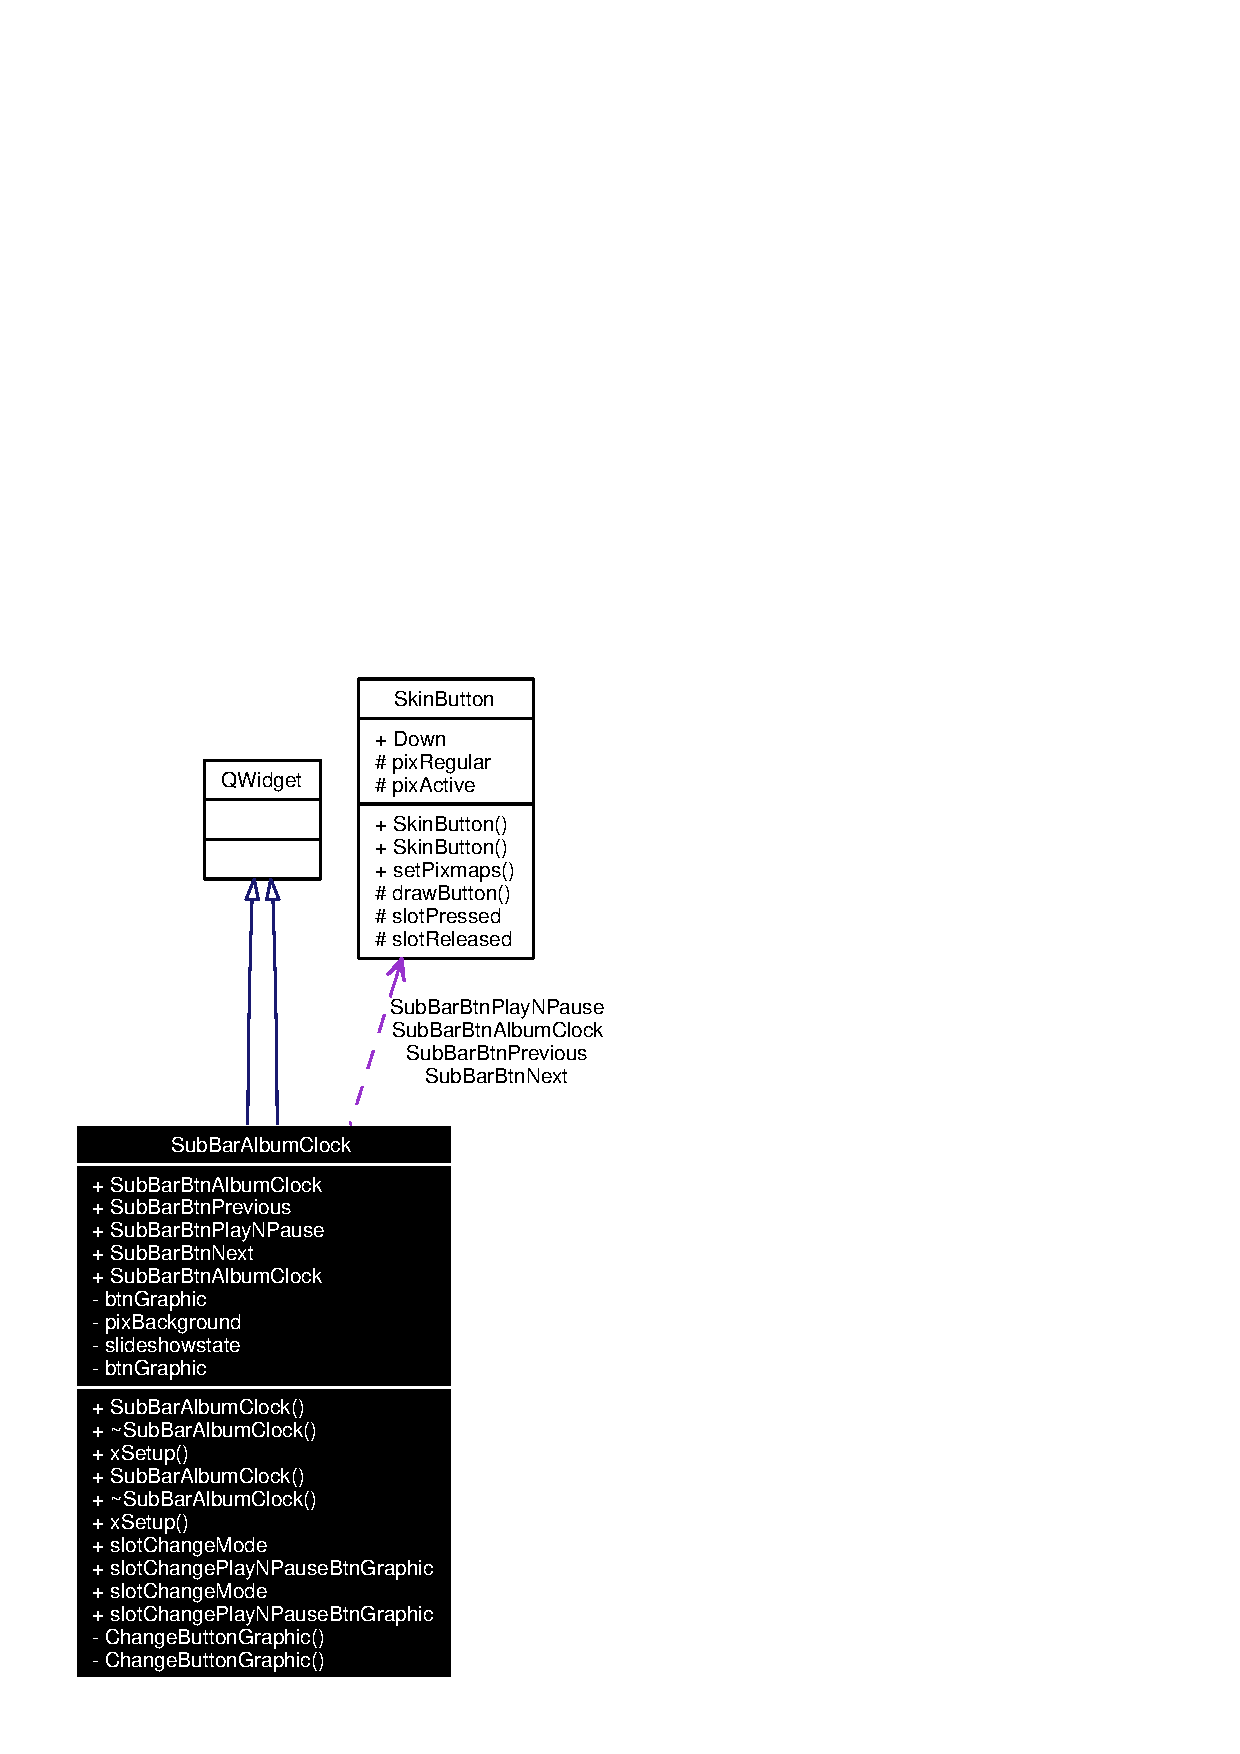
\includegraphics[width=159pt]{classSubBarAlbumClock__coll__graph}
\end{center}
\end{figure}


\subsection{Detailed Description}
\begin{Desc}
\item[Author:]sonicat \end{Desc}




Definition at line 30 of file src/subbaralbumclock.h.\subsection*{Public Slots}
\begin{CompactItemize}
\item 
void {\bf slot\-Change\-Mode} ()
\item 
void {\bf slot\-Change\-Play\-NPause\-Btn\-Graphic} ()
\item 
void {\bf slot\-Change\-Mode} ()
\item 
void {\bf slot\-Change\-Play\-NPause\-Btn\-Graphic} ()
\end{CompactItemize}
\subsection*{Signals}
\begin{CompactItemize}
\item 
void {\bf signal\-Album\-Clock\-Mode\-Change\-To\-Dispaly\-Area} (int)
\item 
void {\bf signal\-Album\-Clock\-Mode\-Change\-To\-Dispaly\-Area} (int)
\end{CompactItemize}
\subsection*{Public Member Functions}
\begin{CompactItemize}
\item 
{\bf Sub\-Bar\-Album\-Clock} ({\bf QWidget} $\ast$parent=0, const char $\ast$name=0)
\item 
{\bf $\sim$Sub\-Bar\-Album\-Clock} ()
\item 
void {\bf x\-Setup} ()
\item 
{\bf Sub\-Bar\-Album\-Clock} ({\bf QWidget} $\ast$parent=0, const char $\ast$name=0)
\item 
{\bf $\sim$Sub\-Bar\-Album\-Clock} ()
\item 
void {\bf x\-Setup} ()
\end{CompactItemize}
\subsection*{Public Attributes}
\begin{CompactItemize}
\item 
{\bf Skin\-Button} $\ast$ {\bf Sub\-Bar\-Btn\-Album\-Clock}
\item 
{\bf Skin\-Button} $\ast$ {\bf Sub\-Bar\-Btn\-Previous}
\item 
{\bf Skin\-Button} $\ast$ {\bf Sub\-Bar\-Btn\-Play\-NPause}
\item 
{\bf Skin\-Button} $\ast$ {\bf Sub\-Bar\-Btn\-Next}
\item 
{\bf Skin\-Button} $\ast$ {\bf Sub\-Bar\-Btn\-Album\-Clock}
\end{CompactItemize}
\subsection*{Private Types}
\begin{CompactItemize}
\item 
enum {\bf SLIDESHOWSTATE} \{ {\bf GO} = 0, 
{\bf STOP}
 \}
\item 
enum {\bf SLIDESHOWSTATE} \{ {\bf GO} = 0, 
{\bf STOP}
 \}
\end{CompactItemize}
\subsection*{Private Member Functions}
\begin{CompactItemize}
\item 
void {\bf Change\-Button\-Graphic} (int)
\item 
void {\bf Change\-Button\-Graphic} (int)
\end{CompactItemize}
\subsection*{Private Attributes}
\begin{CompactItemize}
\item 
QPixmap $\ast$ {\bf btn\-Graphic} [12]
\item 
QPixmap {\bf pix\-Background}
\item 
{\bf SLIDESHOWSTATE} {\bf slideshowstate}
\item 
QPixmap $\ast$ {\bf btn\-Graphic} [12]
\end{CompactItemize}


\subsection{Member Enumeration Documentation}
\index{SubBarAlbumClock@{Sub\-Bar\-Album\-Clock}!SLIDESHOWSTATE@{SLIDESHOWSTATE}}
\index{SLIDESHOWSTATE@{SLIDESHOWSTATE}!SubBarAlbumClock@{Sub\-Bar\-Album\-Clock}}
\subsubsection{\setlength{\rightskip}{0pt plus 5cm}enum {\bf Sub\-Bar\-Album\-Clock::SLIDESHOWSTATE}\hspace{0.3cm}{\tt  [private]}}\label{classSubBarAlbumClock_SubBarAlbumClocky3}


\begin{Desc}
\item[Enumeration values: ]\par
\begin{description}
\index{GO@{GO}!SubBarAlbumClock@{SubBarAlbumClock}}\index{SubBarAlbumClock@{SubBarAlbumClock}!GO@{GO}}\item[{\em 
GO\label{classSubBarAlbumClock_SubBarAlbumClocky3SubBarAlbumClocky0}
}]\index{STOP@{STOP}!SubBarAlbumClock@{SubBarAlbumClock}}\index{SubBarAlbumClock@{SubBarAlbumClock}!STOP@{STOP}}\item[{\em 
STOP\label{classSubBarAlbumClock_SubBarAlbumClocky3SubBarAlbumClocky1}
}]\end{description}
\end{Desc}



Definition at line 32 of file subbaralbumclock.h.



\footnotesize\begin{verbatim}33 {
34         GO=0,
35         STOP
36 };
\end{verbatim}\normalsize 
\index{SubBarAlbumClock@{Sub\-Bar\-Album\-Clock}!SLIDESHOWSTATE@{SLIDESHOWSTATE}}
\index{SLIDESHOWSTATE@{SLIDESHOWSTATE}!SubBarAlbumClock@{Sub\-Bar\-Album\-Clock}}
\subsubsection{\setlength{\rightskip}{0pt plus 5cm}enum {\bf Sub\-Bar\-Album\-Clock::SLIDESHOWSTATE}\hspace{0.3cm}{\tt  [private]}}\label{classSubBarAlbumClock_SubBarAlbumClocky2}


\begin{Desc}
\item[Enumeration values: ]\par
\begin{description}
\index{GO@{GO}!SubBarAlbumClock@{SubBarAlbumClock}}\index{SubBarAlbumClock@{SubBarAlbumClock}!GO@{GO}}\item[{\em 
GO\label{classSubBarAlbumClock_SubBarAlbumClocky3SubBarAlbumClocky0}
}]\index{STOP@{STOP}!SubBarAlbumClock@{SubBarAlbumClock}}\index{SubBarAlbumClock@{SubBarAlbumClock}!STOP@{STOP}}\item[{\em 
STOP\label{classSubBarAlbumClock_SubBarAlbumClocky3SubBarAlbumClocky1}
}]\end{description}
\end{Desc}



Definition at line 33 of file src/subbaralbumclock.h.



\footnotesize\begin{verbatim}34 {
35         GO=0,
36         STOP
37 };
\end{verbatim}\normalsize 


\subsection{Constructor \& Destructor Documentation}
\index{SubBarAlbumClock@{Sub\-Bar\-Album\-Clock}!SubBarAlbumClock@{SubBarAlbumClock}}
\index{SubBarAlbumClock@{SubBarAlbumClock}!SubBarAlbumClock@{Sub\-Bar\-Album\-Clock}}
\subsubsection{\setlength{\rightskip}{0pt plus 5cm}Sub\-Bar\-Album\-Clock::Sub\-Bar\-Album\-Clock ({\bf QWidget} $\ast$ {\em parent} = 0, const char $\ast$ {\em name} = 0)}\label{classSubBarAlbumClock_SubBarAlbumClocka0}




Definition at line 22 of file src/subbaralbumclock.cpp.

References x\-Setup().



\footnotesize\begin{verbatim}23  : QWidget(parent, name)
24 {
25  xSetup();
26 }
\end{verbatim}\normalsize 


Here is the call graph for this function:\begin{figure}[H]
\begin{center}
\leavevmode
\includegraphics[width=284pt]{classSubBarAlbumClock_SubBarAlbumClocka0_cgraph}
\end{center}
\end{figure}
\index{SubBarAlbumClock@{Sub\-Bar\-Album\-Clock}!~SubBarAlbumClock@{$\sim$SubBarAlbumClock}}
\index{~SubBarAlbumClock@{$\sim$SubBarAlbumClock}!SubBarAlbumClock@{Sub\-Bar\-Album\-Clock}}
\subsubsection{\setlength{\rightskip}{0pt plus 5cm}Sub\-Bar\-Album\-Clock::$\sim${\bf Sub\-Bar\-Album\-Clock} ()}\label{classSubBarAlbumClock_SubBarAlbumClocka1}




Definition at line 29 of file src/subbaralbumclock.cpp.



\footnotesize\begin{verbatim}30 {
31 }
\end{verbatim}\normalsize 
\index{SubBarAlbumClock@{Sub\-Bar\-Album\-Clock}!SubBarAlbumClock@{SubBarAlbumClock}}
\index{SubBarAlbumClock@{SubBarAlbumClock}!SubBarAlbumClock@{Sub\-Bar\-Album\-Clock}}
\subsubsection{\setlength{\rightskip}{0pt plus 5cm}Sub\-Bar\-Album\-Clock::Sub\-Bar\-Album\-Clock ({\bf QWidget} $\ast$ {\em parent} = 0, const char $\ast$ {\em name} = 0)}\label{classSubBarAlbumClock_SubBarAlbumClocka3}


\index{SubBarAlbumClock@{Sub\-Bar\-Album\-Clock}!~SubBarAlbumClock@{$\sim$SubBarAlbumClock}}
\index{~SubBarAlbumClock@{$\sim$SubBarAlbumClock}!SubBarAlbumClock@{Sub\-Bar\-Album\-Clock}}
\subsubsection{\setlength{\rightskip}{0pt plus 5cm}Sub\-Bar\-Album\-Clock::$\sim${\bf Sub\-Bar\-Album\-Clock} ()}\label{classSubBarAlbumClock_SubBarAlbumClocka4}




\subsection{Member Function Documentation}
\index{SubBarAlbumClock@{Sub\-Bar\-Album\-Clock}!ChangeButtonGraphic@{ChangeButtonGraphic}}
\index{ChangeButtonGraphic@{ChangeButtonGraphic}!SubBarAlbumClock@{Sub\-Bar\-Album\-Clock}}
\subsubsection{\setlength{\rightskip}{0pt plus 5cm}void Sub\-Bar\-Album\-Clock::Change\-Button\-Graphic (int)\hspace{0.3cm}{\tt  [private]}}\label{classSubBarAlbumClock_SubBarAlbumClockd1}


\index{SubBarAlbumClock@{Sub\-Bar\-Album\-Clock}!ChangeButtonGraphic@{ChangeButtonGraphic}}
\index{ChangeButtonGraphic@{ChangeButtonGraphic}!SubBarAlbumClock@{Sub\-Bar\-Album\-Clock}}
\subsubsection{\setlength{\rightskip}{0pt plus 5cm}void Sub\-Bar\-Album\-Clock::Change\-Button\-Graphic (int)\hspace{0.3cm}{\tt  [private]}}\label{classSubBarAlbumClock_SubBarAlbumClockd0}




Definition at line 89 of file src/subbaralbumclock.cpp.

References Global\-Setting, HDASSGlobal\-Setting::int\-HDSS\_\-DISPLAY\_\-STATE, Skin\-Button::set\-Pixmaps(), signal\-Album\-Clock\-Mode\-Change\-To\-Dispaly\-Area(), and Sub\-Bar\-Btn\-Album\-Clock.

Referenced by slot\-Change\-Mode().



\footnotesize\begin{verbatim}90 {
91     qWarning("~~~~~~~~%d",GlobalSetting.intHDSS_DISPLAY_STATE);
92     emit signalAlbumClockModeChangeToDispalyArea(GlobalSetting.intHDSS_DISPLAY_STATE);
93    if(!Mode)//Album
94    SubBarBtnAlbumClock->setPixmaps(btnGraphic[0],btnGraphic[1]);
95    else//Clock
96    SubBarBtnAlbumClock->setPixmaps(btnGraphic[2],btnGraphic[3]);
97  
98 }
\end{verbatim}\normalsize 


Here is the call graph for this function:\begin{figure}[H]
\begin{center}
\leavevmode
\includegraphics[width=202pt]{classSubBarAlbumClock_SubBarAlbumClockd0_cgraph}
\end{center}
\end{figure}
\index{SubBarAlbumClock@{Sub\-Bar\-Album\-Clock}!signalAlbumClockModeChangeToDispalyArea@{signalAlbumClockModeChangeToDispalyArea}}
\index{signalAlbumClockModeChangeToDispalyArea@{signalAlbumClockModeChangeToDispalyArea}!SubBarAlbumClock@{Sub\-Bar\-Album\-Clock}}
\subsubsection{\setlength{\rightskip}{0pt plus 5cm}void Sub\-Bar\-Album\-Clock::signal\-Album\-Clock\-Mode\-Change\-To\-Dispaly\-Area (int)\hspace{0.3cm}{\tt  [signal]}}\label{classSubBarAlbumClock_SubBarAlbumClockl1}


\index{SubBarAlbumClock@{Sub\-Bar\-Album\-Clock}!signalAlbumClockModeChangeToDispalyArea@{signalAlbumClockModeChangeToDispalyArea}}
\index{signalAlbumClockModeChangeToDispalyArea@{signalAlbumClockModeChangeToDispalyArea}!SubBarAlbumClock@{Sub\-Bar\-Album\-Clock}}
\subsubsection{\setlength{\rightskip}{0pt plus 5cm}void Sub\-Bar\-Album\-Clock::signal\-Album\-Clock\-Mode\-Change\-To\-Dispaly\-Area (int)\hspace{0.3cm}{\tt  [signal]}}\label{classSubBarAlbumClock_SubBarAlbumClockl0}




Definition at line 89 of file subbaralbumclock.moc.

Referenced by Change\-Button\-Graphic().



\footnotesize\begin{verbatim}90 {
91     activate_signal( staticMetaObject()->signalOffset() + 0, t0 );
92 }
\end{verbatim}\normalsize 
\index{SubBarAlbumClock@{Sub\-Bar\-Album\-Clock}!slotChangeMode@{slotChangeMode}}
\index{slotChangeMode@{slotChangeMode}!SubBarAlbumClock@{Sub\-Bar\-Album\-Clock}}
\subsubsection{\setlength{\rightskip}{0pt plus 5cm}void Sub\-Bar\-Album\-Clock::slot\-Change\-Mode ()\hspace{0.3cm}{\tt  [slot]}}\label{classSubBarAlbumClock_SubBarAlbumClocki2}


\index{SubBarAlbumClock@{Sub\-Bar\-Album\-Clock}!slotChangeMode@{slotChangeMode}}
\index{slotChangeMode@{slotChangeMode}!SubBarAlbumClock@{Sub\-Bar\-Album\-Clock}}
\subsubsection{\setlength{\rightskip}{0pt plus 5cm}void Sub\-Bar\-Album\-Clock::slot\-Change\-Mode ()\hspace{0.3cm}{\tt  [slot]}}\label{classSubBarAlbumClock_SubBarAlbumClocki0}




Definition at line 78 of file src/subbaralbumclock.cpp.

References Change\-Button\-Graphic(), Global\-Setting, HDASSGlobal\-Setting::int\-HDASS\_\-ALBUMCLOCK\_\-STATE, and HDASSGlobal\-Setting::int\-HDSS\_\-DISPLAY\_\-STATE.

Referenced by x\-Setup().



\footnotesize\begin{verbatim}79 {
80   
81   // +3 make the value init form em_dispaly_album (3)
82   //qWarning("~~~~~~~~%d",GlobalSetting.intHDASS_ALBUMCLOCK_STATE);
83   GlobalSetting.intHDASS_ALBUMCLOCK_STATE++;
84   GlobalSetting.intHDASS_ALBUMCLOCK_STATE%=2;
85   GlobalSetting.intHDSS_DISPLAY_STATE=GlobalSetting.intHDASS_ALBUMCLOCK_STATE+3;
86   ChangeButtonGraphic(GlobalSetting.intHDASS_ALBUMCLOCK_STATE);
87 }
\end{verbatim}\normalsize 
\index{SubBarAlbumClock@{Sub\-Bar\-Album\-Clock}!slotChangePlayNPauseBtnGraphic@{slotChangePlayNPauseBtnGraphic}}
\index{slotChangePlayNPauseBtnGraphic@{slotChangePlayNPauseBtnGraphic}!SubBarAlbumClock@{Sub\-Bar\-Album\-Clock}}
\subsubsection{\setlength{\rightskip}{0pt plus 5cm}void Sub\-Bar\-Album\-Clock::slot\-Change\-Play\-NPause\-Btn\-Graphic ()\hspace{0.3cm}{\tt  [slot]}}\label{classSubBarAlbumClock_SubBarAlbumClocki3}


\index{SubBarAlbumClock@{Sub\-Bar\-Album\-Clock}!slotChangePlayNPauseBtnGraphic@{slotChangePlayNPauseBtnGraphic}}
\index{slotChangePlayNPauseBtnGraphic@{slotChangePlayNPauseBtnGraphic}!SubBarAlbumClock@{Sub\-Bar\-Album\-Clock}}
\subsubsection{\setlength{\rightskip}{0pt plus 5cm}void Sub\-Bar\-Album\-Clock::slot\-Change\-Play\-NPause\-Btn\-Graphic ()\hspace{0.3cm}{\tt  [slot]}}\label{classSubBarAlbumClock_SubBarAlbumClocki1}




Definition at line 100 of file src/subbaralbumclock.cpp.

References GO, Skin\-Button::set\-Pixmaps(), slideshowstate, STOP, and Sub\-Bar\-Btn\-Play\-NPause.

Referenced by x\-Setup().



\footnotesize\begin{verbatim}101 {
102   if(slideshowstate==SubBarAlbumClock::STOP)
103  {
104   slideshowstate=SubBarAlbumClock::GO;
105   SubBarBtnPlayNPause->setPixmaps(btnGraphic[6],btnGraphic[7]);
106  }
107  else
108  {
109   slideshowstate=SubBarAlbumClock::STOP;
110   SubBarBtnPlayNPause->setPixmaps(btnGraphic[8],btnGraphic[9]);
111  }
112 }
\end{verbatim}\normalsize 
\index{SubBarAlbumClock@{Sub\-Bar\-Album\-Clock}!xSetup@{xSetup}}
\index{xSetup@{xSetup}!SubBarAlbumClock@{Sub\-Bar\-Album\-Clock}}
\subsubsection{\setlength{\rightskip}{0pt plus 5cm}void Sub\-Bar\-Album\-Clock::x\-Setup ()}\label{classSubBarAlbumClock_SubBarAlbumClocka5}


\index{SubBarAlbumClock@{Sub\-Bar\-Album\-Clock}!xSetup@{xSetup}}
\index{xSetup@{xSetup}!SubBarAlbumClock@{Sub\-Bar\-Album\-Clock}}
\subsubsection{\setlength{\rightskip}{0pt plus 5cm}void Sub\-Bar\-Album\-Clock::x\-Setup ()}\label{classSubBarAlbumClock_SubBarAlbumClocka2}




Definition at line 32 of file src/subbaralbumclock.cpp.

References Skin\-Button::set\-Pixmaps(), slot\-Change\-Mode(), slot\-Change\-Play\-NPause\-Btn\-Graphic(), Sub\-Bar\-Btn\-Album\-Clock, Sub\-Bar\-Btn\-Next, Sub\-Bar\-Btn\-Play\-NPause, and Sub\-Bar\-Btn\-Previous.

Referenced by Sub\-Bar\-Album\-Clock().



\footnotesize\begin{verbatim}33 {
34    //DAVID Setup Background;
35    pixBackground.load("/root/kde_application/hdass08/skin/SubBarBackground.png");
36    setBackgroundPixmap(pixBackground);
37    
38    //InitBtn Graphic
39    btnGraphic[0]=new QPixmap("/root/kde_application/hdass08/skin/Bar-Album-Btn-Album.png");
40    btnGraphic[1]=new QPixmap("/root/kde_application/hdass08/skin/Bar-Album-Btn-Album-Active.png");
41    btnGraphic[2]=new QPixmap("/root/kde_application/hdass08/skin/Bar-Album-Btn-Clock.png");
42    btnGraphic[3]=new QPixmap("/root/kde_application/hdass08/skin/Bar-Album-Btn-Clock-Active.png");
43    btnGraphic[4]=new QPixmap("/root/kde_application/hdass08/skin/Bar-Album-Btn-Previous.png");
44    btnGraphic[5]=new QPixmap("/root/kde_application/hdass08/skin/Bar-Album-Btn-Previous-Active.png");
45    btnGraphic[6]=new QPixmap("/root/kde_application/hdass08/skin/Bar-Album-Btn-Play.png");
46    btnGraphic[7]=new QPixmap("/root/kde_application/hdass08/skin/Bar-Album-Btn-Play-Active.png");
47    btnGraphic[8]=new QPixmap("/root/kde_application/hdass08/skin/Bar-Album-Btn-Pause.png");
48    btnGraphic[9]=new QPixmap("/root/kde_application/hdass08/skin/Bar-Album-Btn-Pause-Active.png");
49    btnGraphic[10]=new QPixmap("/root/kde_application/hdass08/skin/Bar-Album-Btn-Next.png");
50    btnGraphic[11]=new QPixmap("/root/kde_application/hdass08/skin/Bar-Album-Btn-Next-Active.png");
51    //Init Btn
52    SubBarBtnAlbumClock=new SkinButton(this);
53    SubBarBtnAlbumClock->setPixmaps(btnGraphic[0],btnGraphic[1]);
54    SubBarBtnAlbumClock->setGeometry(457,0,80,80);
55    SubBarBtnAlbumClock->show();
56    
57    SubBarBtnPrevious=new SkinButton(this);
58    SubBarBtnPrevious->setPixmaps(btnGraphic[4],btnGraphic[5]);
59    SubBarBtnPrevious->setGeometry(175,0,60,80);
60    SubBarBtnPrevious->show();
61    
62    SubBarBtnPlayNPause=new SkinButton(this);
63    SubBarBtnPlayNPause->setPixmaps(btnGraphic[6],btnGraphic[7]);
64    SubBarBtnPlayNPause->setGeometry(240,0,80,80);
65    SubBarBtnPlayNPause->show();
66    
67    SubBarBtnNext=new SkinButton(this);
68    SubBarBtnNext->setPixmaps(btnGraphic[10],btnGraphic[11]);
69    SubBarBtnNext->setGeometry(323,0,60,80);
70    SubBarBtnNext->show();
71    
72    QObject::connect(SubBarBtnAlbumClock,SIGNAL(pressed()),this,SLOT(slotChangeMode()));
73    QObject::connect(SubBarBtnPlayNPause,SIGNAL(pressed()),this,SLOT(slotChangePlayNPauseBtnGraphic()));
74   // slideshowstate=AlbumControl::GO;
75 
76 }
\end{verbatim}\normalsize 


Here is the call graph for this function:\begin{figure}[H]
\begin{center}
\leavevmode
\includegraphics[width=168pt]{classSubBarAlbumClock_SubBarAlbumClocka2_cgraph}
\end{center}
\end{figure}


\subsection{Member Data Documentation}
\index{SubBarAlbumClock@{Sub\-Bar\-Album\-Clock}!btnGraphic@{btnGraphic}}
\index{btnGraphic@{btnGraphic}!SubBarAlbumClock@{Sub\-Bar\-Album\-Clock}}
\subsubsection{\setlength{\rightskip}{0pt plus 5cm}QPixmap$\ast$ {\bf Sub\-Bar\-Album\-Clock::btn\-Graphic}[12]\hspace{0.3cm}{\tt  [private]}}\label{classSubBarAlbumClock_SubBarAlbumClockr3}




Definition at line 52 of file subbaralbumclock.h.\index{SubBarAlbumClock@{Sub\-Bar\-Album\-Clock}!btnGraphic@{btnGraphic}}
\index{btnGraphic@{btnGraphic}!SubBarAlbumClock@{Sub\-Bar\-Album\-Clock}}
\subsubsection{\setlength{\rightskip}{0pt plus 5cm}QPixmap$\ast$ {\bf Sub\-Bar\-Album\-Clock::btn\-Graphic}[12]\hspace{0.3cm}{\tt  [private]}}\label{classSubBarAlbumClock_SubBarAlbumClockr0}




Definition at line 52 of file src/subbaralbumclock.h.\index{SubBarAlbumClock@{Sub\-Bar\-Album\-Clock}!pixBackground@{pixBackground}}
\index{pixBackground@{pixBackground}!SubBarAlbumClock@{Sub\-Bar\-Album\-Clock}}
\subsubsection{\setlength{\rightskip}{0pt plus 5cm}QPixmap {\bf Sub\-Bar\-Album\-Clock::pix\-Background}\hspace{0.3cm}{\tt  [private]}}\label{classSubBarAlbumClock_SubBarAlbumClockr1}




Definition at line 53 of file subbaralbumclock.h.\index{SubBarAlbumClock@{Sub\-Bar\-Album\-Clock}!slideshowstate@{slideshowstate}}
\index{slideshowstate@{slideshowstate}!SubBarAlbumClock@{Sub\-Bar\-Album\-Clock}}
\subsubsection{\setlength{\rightskip}{0pt plus 5cm}{\bf SLIDESHOWSTATE} {\bf Sub\-Bar\-Album\-Clock::slideshowstate}\hspace{0.3cm}{\tt  [private]}}\label{classSubBarAlbumClock_SubBarAlbumClockr2}




Definition at line 55 of file subbaralbumclock.h.

Referenced by slot\-Change\-Play\-NPause\-Btn\-Graphic().\index{SubBarAlbumClock@{Sub\-Bar\-Album\-Clock}!SubBarBtnAlbumClock@{SubBarBtnAlbumClock}}
\index{SubBarBtnAlbumClock@{SubBarBtnAlbumClock}!SubBarAlbumClock@{Sub\-Bar\-Album\-Clock}}
\subsubsection{\setlength{\rightskip}{0pt plus 5cm}{\bf Skin\-Button}$\ast$ {\bf Sub\-Bar\-Album\-Clock::Sub\-Bar\-Btn\-Album\-Clock}}\label{classSubBarAlbumClock_SubBarAlbumClocko4}




Definition at line 43 of file subbaralbumclock.h.\index{SubBarAlbumClock@{Sub\-Bar\-Album\-Clock}!SubBarBtnAlbumClock@{SubBarBtnAlbumClock}}
\index{SubBarBtnAlbumClock@{SubBarBtnAlbumClock}!SubBarAlbumClock@{Sub\-Bar\-Album\-Clock}}
\subsubsection{\setlength{\rightskip}{0pt plus 5cm}{\bf Skin\-Button}$\ast$ {\bf Sub\-Bar\-Album\-Clock::Sub\-Bar\-Btn\-Album\-Clock}}\label{classSubBarAlbumClock_SubBarAlbumClocko0}




Definition at line 43 of file src/subbaralbumclock.h.

Referenced by Change\-Button\-Graphic(), and x\-Setup().\index{SubBarAlbumClock@{Sub\-Bar\-Album\-Clock}!SubBarBtnNext@{SubBarBtnNext}}
\index{SubBarBtnNext@{SubBarBtnNext}!SubBarAlbumClock@{Sub\-Bar\-Album\-Clock}}
\subsubsection{\setlength{\rightskip}{0pt plus 5cm}{\bf Skin\-Button} $\ast$ {\bf Sub\-Bar\-Album\-Clock::Sub\-Bar\-Btn\-Next}}\label{classSubBarAlbumClock_SubBarAlbumClocko3}




Definition at line 43 of file subbaralbumclock.h.

Referenced by x\-Setup(), and HDASS08::x\-Setup().\index{SubBarAlbumClock@{Sub\-Bar\-Album\-Clock}!SubBarBtnPlayNPause@{SubBarBtnPlayNPause}}
\index{SubBarBtnPlayNPause@{SubBarBtnPlayNPause}!SubBarAlbumClock@{Sub\-Bar\-Album\-Clock}}
\subsubsection{\setlength{\rightskip}{0pt plus 5cm}{\bf Skin\-Button} $\ast$ {\bf Sub\-Bar\-Album\-Clock::Sub\-Bar\-Btn\-Play\-NPause}}\label{classSubBarAlbumClock_SubBarAlbumClocko2}




Definition at line 43 of file subbaralbumclock.h.

Referenced by slot\-Change\-Play\-NPause\-Btn\-Graphic(), x\-Setup(), and HDASS08::x\-Setup().\index{SubBarAlbumClock@{Sub\-Bar\-Album\-Clock}!SubBarBtnPrevious@{SubBarBtnPrevious}}
\index{SubBarBtnPrevious@{SubBarBtnPrevious}!SubBarAlbumClock@{Sub\-Bar\-Album\-Clock}}
\subsubsection{\setlength{\rightskip}{0pt plus 5cm}{\bf Skin\-Button} $\ast$ {\bf Sub\-Bar\-Album\-Clock::Sub\-Bar\-Btn\-Previous}}\label{classSubBarAlbumClock_SubBarAlbumClocko1}




Definition at line 43 of file subbaralbumclock.h.

Referenced by x\-Setup(), and HDASS08::x\-Setup().

The documentation for this class was generated from the following files:\begin{CompactItemize}
\item 
{\bf src/subbaralbumclock.h}\item 
{\bf subbaralbumclock.h}\item 
{\bf subbaralbumclock.moc}\item 
{\bf src/subbaralbumclock.cpp}\item 
{\bf subbaralbumclock.cpp}\end{CompactItemize}
